
\documentclass[12pt,a4paper]{article}

\usepackage[utf8]{inputenc}
\usepackage[T1]{fontenc}
\usepackage{polski}

\usepackage{amsthm}
\usepackage{amsmath}
\usepackage{amsfonts}
\usepackage{amssymb}
\usepackage{pgfplots}
\usepackage{tikz}
\usepackage{lmodern}	%fancy font
\usepackage{textcomp}

\usepackage{indentfirst}
\usepackage{graphicx}
\usepackage{caption}
\usepackage{subcaption}
%\usepackage{siunitx}
\usepackage{here}


\setlength{\textheight}{24cm}
\setlength{\textwidth}{15.92cm}
\setlength{\footskip}{10mm}
\setlength{\oddsidemargin}{0mm}
\setlength{\evensidemargin}{0mm}
\setlength{\topmargin}{0mm}
\setlength{\headsep}{5mm}
\usepackage{tikz}
\usepackage{lmodern}	%fancy font
\usepackage{textcomp}

\usepackage{indentfirst}
\usepackage{graphicx}
\usepackage{caption}
\usepackage{subcaption}
%\usepackage{siunitx}
\usepackage{here}
\usepackage[margin=1in]{geometry}% Just for this example
\setlength{\parindent}{0pt}% Just for this example
\setlength{\textheight}{24cm}
\setlength{\textwidth}{15.92cm}
\setlength{\footskip}{10mm}
\setlength{\oddsidemargin}{0mm}
\setlength{\evensidemargin}{0mm}
\setlength{\topmargin}{0mm}


\begin{document}

\begin{table}[]
\label{my-label}
\begin{tabular}{|p{7.5cm}|p{7.5cm}|}
\hline
									           					&                           \\

\includegraphics[height=3cm]{logo}             					& \textbf{Technika cyfrowa} \\ \hline
\multicolumn{1}{|l|}{\textbf{Temat ćwiczenia}} 					& \textbf{Numer ćwiczenia}  \\
\multicolumn{1}{|l|}{Liczniki}	& 2                         \\ \hline
\multicolumn{1}{|l|}{\textbf{Wykonawca}}       & \textbf{Ocena}            \\
\multicolumn{1}{|l|}{Marcin Przewięźlikowski}          &                           \\ \hline
\end{tabular}
\end{table}

\section{Cel ćwiczenia}

Zapoznanie się z zastosowaniem przerzutników w budowaniu liczników synchronicznych oraz asynchronicznych. Zbadanie działania liczników czterobitowych.

\section{Dwójka licząca}


Dwójka licząca służy do dzielenia częstotliwości sygnału wejściowego przez 2. Uzyskano ją na dwa sposoby:

\subsection{Przerzutnik D}


Dwójka licząca służy do dzielenia częstotliwości sygnału wejściowego przez 2. Oto jej tabela prawdy:



\begin{figure}[H]
\centering
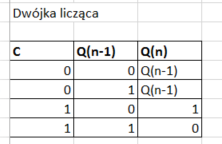
\includegraphics{img/4a_table}
\end{figure}

Uzyskano ją na dwa sposoby:

\begin{figure}[H]
\centering
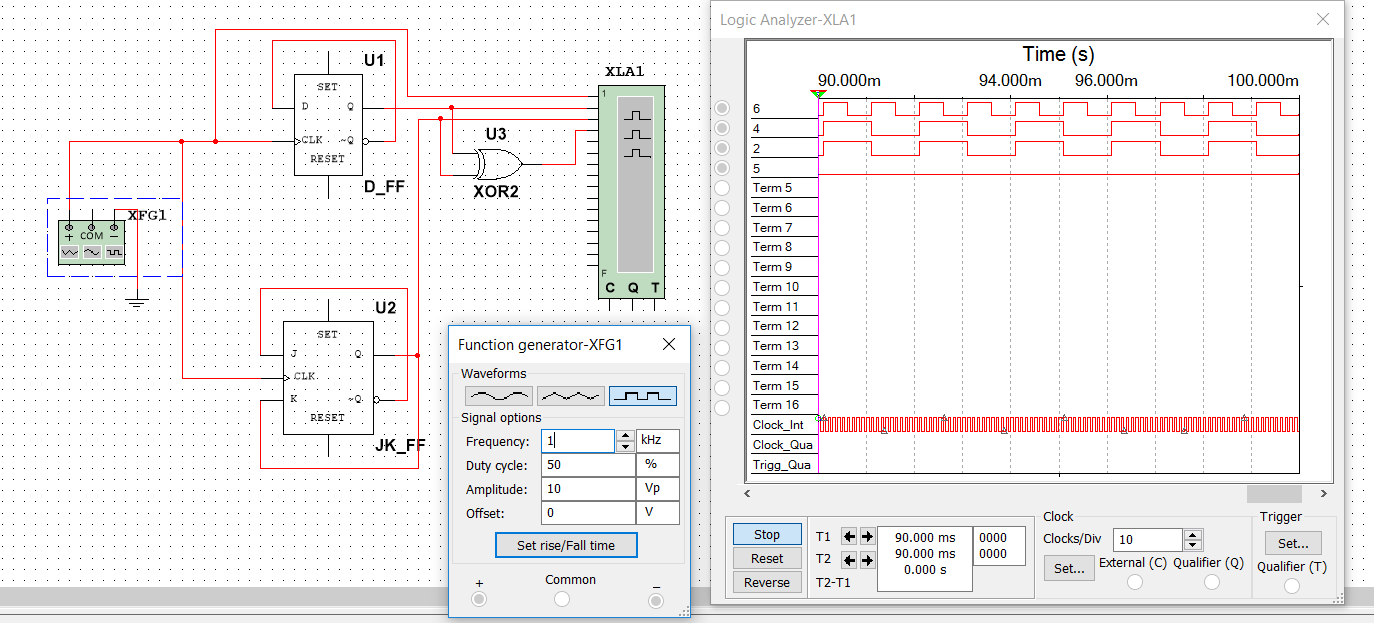
\includegraphics[width=\textwidth]{img/4a}
\end{figure}

\subsection{Przerzutnik D}
\begin{figure}[H]
\centering
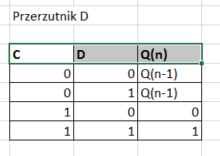
\includegraphics{img/4a_table_d}
\end{figure}
Chcemy, aby wartość logiczna Q zmieniała się na przeciwną niż dotychczasowa tylko, gdy sygnał zegara jest wzrastający.

Właściwości przerzutnika D, pozwalają na uzyskanie zmiany wartości wyjścia na wartość podaną na wejście D tylko, gdy sygnał zegara jest wzrastający. Jak jednak uzyskać zmianę sygnału na wręcz przeciwny? 
Na wejście D trzeba podać zanegowanie obecnej wartości sygnału Q - czyli -Q.

\subsection{Przerzutnik JK}

\begin{figure}[H]
\centering
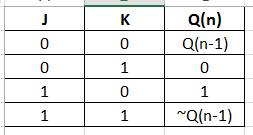
\includegraphics{img/4a_table_jk}
\end{figure}

Wyjście przerzutnika JK zmienia swój stan tylko wtedy, gdy sygnał zegara jest wzrastający. Ponadto, sygnał wyjściowy jest ustawiany zawsze na wartość wejścia J, gdy na wejścia J i K są podane przeciwne sygnały. 

W związku z tym wystarczy na wejście K podać sygnał wyjściowy (Q), a na wejście J - zanegowany sygnał wyjściowy (-Q). Mamy wtedy gwarancję, że sygnał przerzutnika zmieni się na wartość przeciwną do dotychczasowej.

\section{Czterobitowy licznik asynchroniczny}

Do budowy czterobitowego licznika użyto dwójek liczących stworzonych za pomocą przerzutników typu T ze stale podanym na wejście T sygnałem dodatnim. Sprawia to, że przerzutniki reagują zmianą sygnału wyjściowego na wzrastający sygnał zegara.
\par
Tym sposobem każdy licznik dzieli częstotliwość sygnału otrzymywanego na wyjściu C przez 2. 

\begin{figure}[H]
\centering
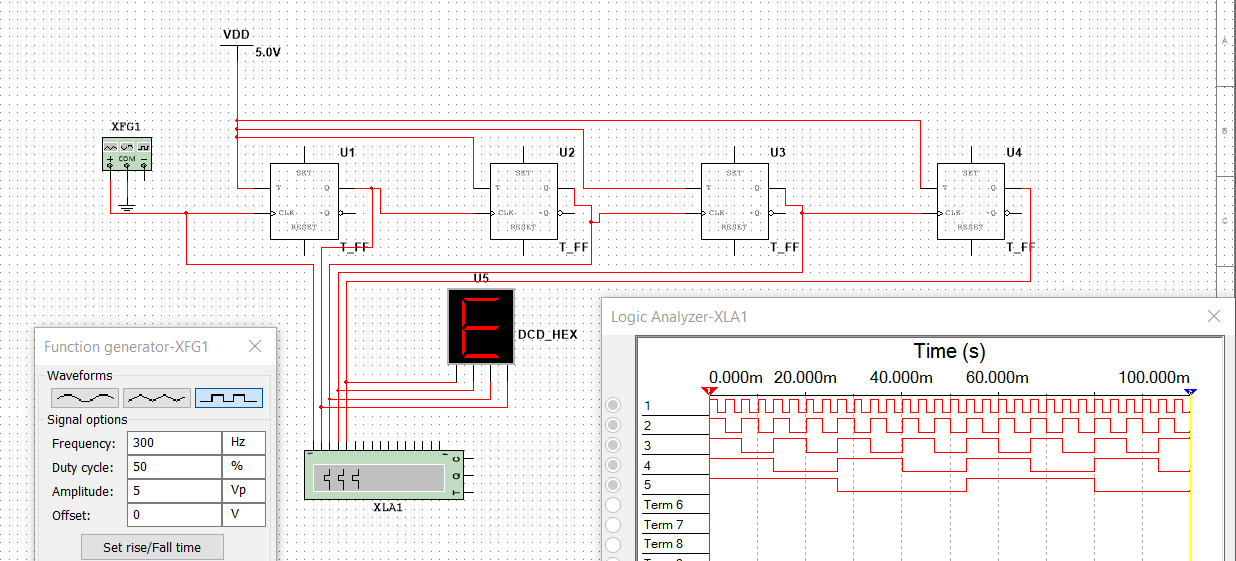
\includegraphics[width=\textwidth]{img/4b_wzrost}
\end{figure}

Zauważono następującą zależność sygnałów na wyjściu od liczby sygnałów z zegara na wejściu:

\begin{figure}[H]
\centering
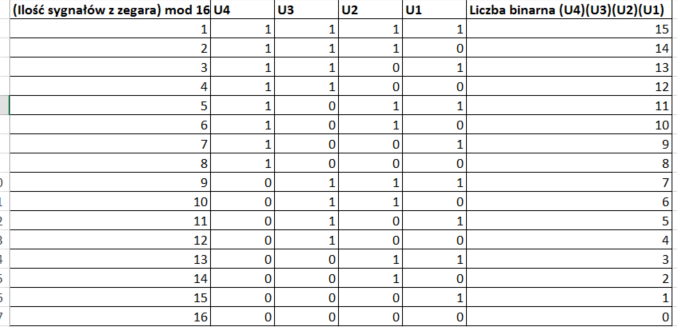
\includegraphics[width=\textwidth]{img/4b_wzrost_table}
\end{figure}

- liczba na wyjściu jest równa 16 - (liczba sygnałów z zegara mod 16)
\par
\par 
Zrealizowano także układ w oparciu o dwójki liczące reagujące na sygnał opadający z zegara. W tym celu na wejście każdego z przerzutników T w układzie dodano bramkę NOT. 
Wtedy, gdy na wejściu bramki NOT jest sygnał opadający, podaje ona sygnał wzrastający na wejście przerzutnika T, na który ten reaguje. Efektywnie Układ NOT-T zachowuje się jak bramka T reagująca na sygnał opadający. Tak działająca bramka T również dzieli częstotliwość podanego sygnału przez 2.


\begin{figure}[H]
\centering
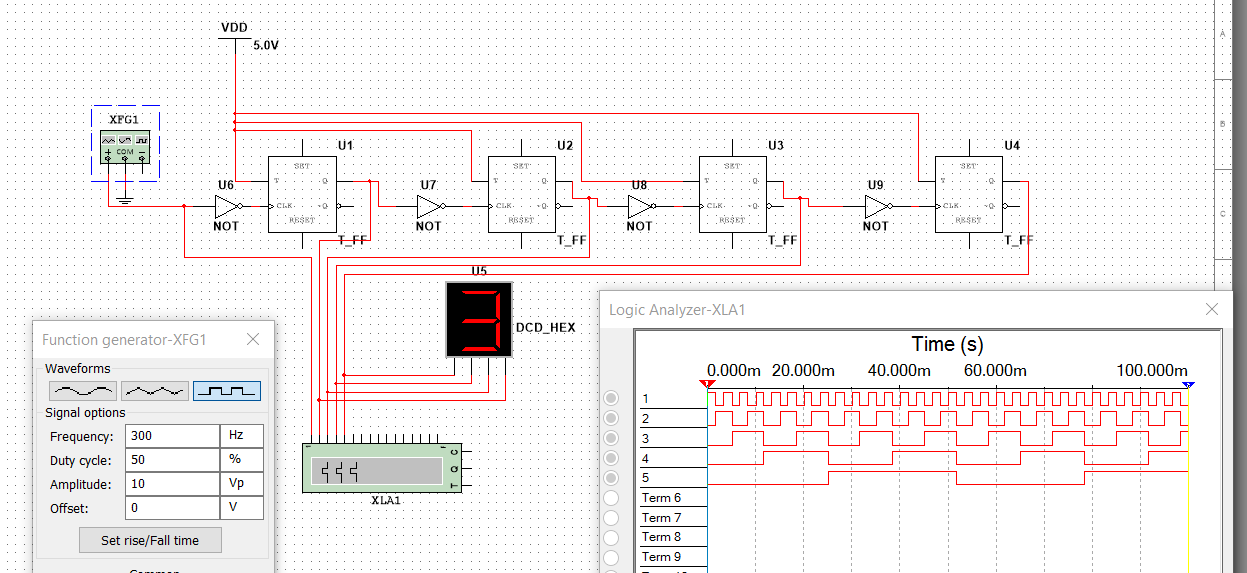
\includegraphics[width=\textwidth]{img/4b_opad}
\end{figure}

Zauważono następującą zależność sygnałów na wyjściu od liczby sygnałów z zegara na wejściu:
\begin{figure}[H]
\centering
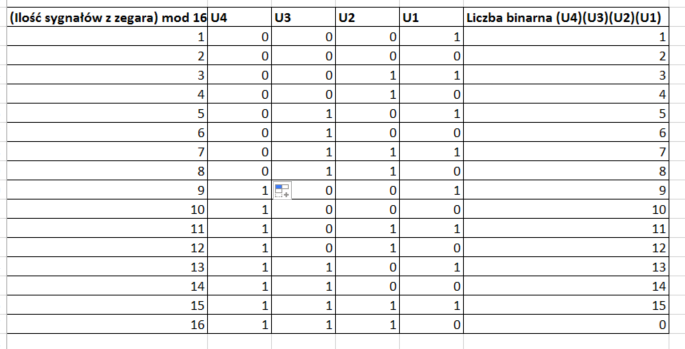
\includegraphics[width=\textwidth]{img/4b_opad_table}
\end{figure}

Widać zatem, że liczba na wyjściu jest równa liczbie sygnałów z zegara mod 16.

\par
Licznik ten nazywamy asynchronicznym, gdyż jego wyjście nie ustala się równocześnie z wejściem, lecz zależy od czasu propagacji sygnału w składowych przerzutnikach. Nie jest to dobre rozwiązanie - jeśli przerzutniki mają duży czas propagacji sygnału, licznik może "gubić" niektóre bity wyjścia lub też po prostu podawać niewłaściwy ich zestaw.

\section{Synchroniczny licznik mod 8}

Liczniki synchroniczne rozwiązują problem liczników asynchronicznych - sygnał zegara jest podawany na każdy z przerzutników osobno, zatem redukuje się czas opóźnień.

Ponieważ licznik jest modulo 8, to wystarczy, by jego wyjście było 3-bitowe.

Rozważmy tabelę prawdy dla każdego z wyjść licznika:

\begin{figure}[H]
\centering
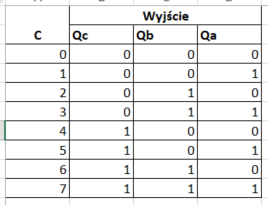
\includegraphics{img/4c_table}
\end{figure}

Można zatem zauważyć, że:
\par
Wyjście Qa zmienia swój stan na przeciwny po każdym impulsie zegarowym.
\par
Wyjście Qb zmienia swój stan na przeciwny po sygnale zegarowym, w czasie którego wyjście Qa było w stanie wysokim.
\par 
Wyjście Qc zmienia stan na przeciwny, gdy w poprzednim cyklu licznika wyjścia Qa i Qb jednocześnie były w stanie wysokim.
\par 

Do budowy wyjść Qa, Qb, Qc będzie zatem najłatwiej użyć przerzutników T reagujących na wzrastający sygnał zegara.
Na wejście T przerzutnika Qa podamy stały sygnał wysoki. Na wejście T przerzutnika Qb podamy sygnał wyjściowy przerzutnika Qa (dzięki temu Qb będzie zmieniał sygnał tylko, gdy wyjście Qa jest dodatnie). Zaś na wejście T przerzutnika Qc podamy sygnały z wyjść Qa i Qb połączone bramką AND - dzięki temu Qc będzie zmieniać sygnał tylko, gdy sygnały Qa i Qb są dodatnie. Dzięki temu Na wyjściu otrzymamy liczbę sygnałów pozytywnych z zegara modulo 8:

\begin{figure}[H]
\centering
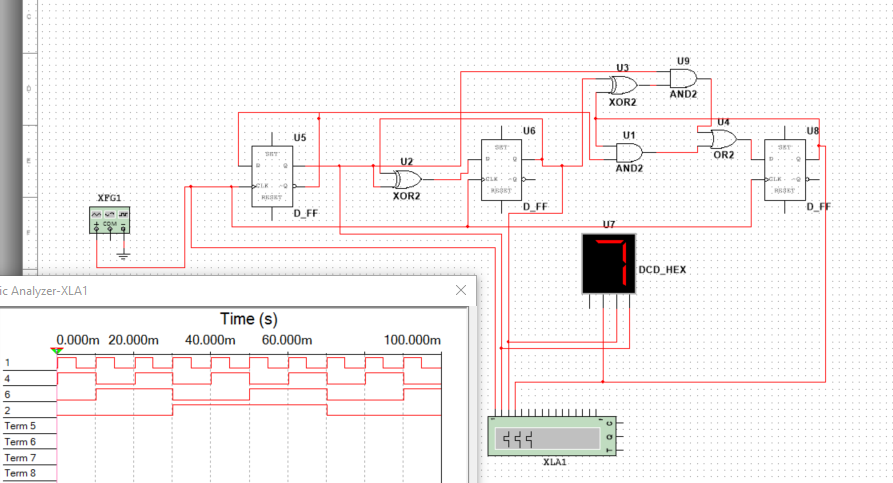
\includegraphics{img/4c}
\end{figure}



\section{Synchroniczny licznik mod 6}




\end{document}
